\documentclass{article}

%% Created with wxMaxima 0.8.4

\setlength{\parskip}{\medskipamount}
\setlength{\parindent}{0pt}
\usepackage[utf8]{inputenc}
\usepackage{graphicx}
\usepackage{amsmath, amssymb}
\usepackage{kotex}

\begin{document}

\pagebreak{}
{\Huge \underline{\sc 
10분에 배우는 wxMaxima}}
\setcounter{section}{0}
\setcounter{subsection}{0}
\setcounter{figure}{0}



방가! 짧은 소개자료를 통해서 wxMaxima와 Maxima의 기초를 배워봅시다. 
맥시마는 매써매티카나 메이플같은 CAS(Computer Algebra System)
소프트웨어입니다. 

하지만 맥시마는 커맨드라인(명령행) 어플리케이션이라 그 보다 나중에 나온
매써매티카나 메이플보다는 `약간' 사용하기 힘들었지요. 그래서 여기 wxMaxima가 
나오게 되는 거지요. 헤헤.  wxMaxima는 맥시마를 위한 GUI로서 맥시마를 
쉽고 재밌게 쓸 수 있습니다.

간단한 계산부터 해볼까요! 아래에 덧셈을 하는 입력 셀이 있습니다. 커서를 옮겨서
SHIFT-ENTER를 눌러 주세요.


\begin{verbatim}
(%i117) 1 + 1;
\end{verbatim}
$$
2\leqno{\tt (\%o117)  }
$$


에러가 안 나오면, 맥시마가 제대로 작동하는 거지요. 에러가 나오면 wxMaxima 설정을
확인하시고, 안되면 wxMaxima(http://wxmaxima.sourceforge.net/)
웹싸이트를 방문하셔서 설치 안내를 확인하셔요.

제대로 작동한다고 가정하고 다음으로 넘어갑니다. 다시 한 번 커서를 옮기셔서
SHIFT-ENTER를 눌러 주세요.


\begin{verbatim}
(%i118) 5!;
% * 10;
%o1 * 100;
1 / 3;
1.0 / 3.0;
\end{verbatim}
$$
120\leqno{\tt (\%o118)  }
$$
$$
1200\leqno{\tt (\%o119)  }
$$
$$
100\\,false\leqno{\tt (\%o120)  }
$$
$$
\frac{1}{3}\leqno{\tt (\%o121)  }
$$
$$
0.33333333333333\leqno{\tt (\%o122)  }
$$


위 입력 셀에서 다섯 줄의 명령을 맥시마에게 보냈습니다. 각 줄은 ``;"나 ``\$"로 끝나야 
합니다. ";"를 쓰시면 맥시마가 출력을 보여드리고, "\$"를 쓰시면 출력이 안 보이지요.
"1/3"이랑 "1.0/3.0"의 결과값이 다른 것에 주의하시고요. 맥시마는 1/3이나 sqrt(2)와 
같은 수식은 계산을 정확하게 하기 위해서 평가를 안 하거든요. ``1.0/3.0"에서는 입력 자체가
(부동소수점을 가진) 소수라서 평가하게 되구요.

그렇지만 원하시면 맥시마에게 (강제로) 부동소수점 계산을 하게 할 수도 있어요. 아래를 
보시지요.


\begin{verbatim}
(%i123) sqrt(2 * %pi);
float(%);
\end{verbatim}
$$
\sqrt{2}\,\sqrt{\pi}\leqno{\tt (\%o123)  }
$$
$$
2.506628274631001\leqno{\tt (\%o124)  }
$$


``float(\%);"를 보시면 ``\%"기호를 썼는 데요. 이 기호는 바로 앞 결과 값을 가집니다.
번호 매겨진 기호 ``\%o1", ``\%o2"\ldots는 입력 셀이 평가될 때마다 그 입력에 대한
출력값을 가집니다. ``variable\_name: value;"를 쓰시면 변수 이름 ``variable\_name"에
``value"를 저장할 수 있는 데요, 변수에는 숫자뿐 아니라 전체 수식을 저장할 수도 있습니다.


\begin{verbatim}
(%i125) radius: 10 $
height: 100 $
area: %pi * radius^2;
volume: area * height;
\end{verbatim}
$$
100\,\pi\leqno{\tt (\%o127)  }
$$
$$
10000\,\pi\leqno{\tt (\%o128)  }
$$


마지막 결과를 평가해볼까요:


\begin{verbatim}
(%i129) float(%);
\end{verbatim}
$$
31415.92653589793\leqno{\tt (\%o129)  }
$$


여태는 맥시마를 그냥 계산기 용도로만 써봤는 데요. 이제 계산기 가지고는 할 수 없는 걸 
해보겠습니다. 부정적분이나 정적분 같은 것 말이죠:


\begin{verbatim}
(%i130) integrate( sin(x), x);
integrate( sin(x), x, 0, %pi);
\end{verbatim}
$$
-cos\left( x\right) \leqno{\tt (\%o130)  }
$$
$$
2\leqno{\tt (\%o131)  }
$$


함수를 하나 정의해서 평가하고 적분해볼까요?


\begin{verbatim}
(%i132) f(x) := x^2 + a$
f(5);
f(5), a = -5;
integrate( f(var), var );
\end{verbatim}
$$
a+25\leqno{\tt (\%o133)  }
$$
$$
20\leqno{\tt (\%o134)  }
$$
$$
\frac{{var}^{3}}{3}+a\,var\leqno{\tt (\%o135)  }
$$


맥시마가 계산하다 헛갈리면, 오히려 질문하기도 합니다. 프롬프트가 저절로 튀어나오면, 질문에
답하셔야 합니다. 답을 쓰시고 다시 한 번 SHIFT-ENTER를 누르셔요. 밑에 질문 보시면 
``positive"인지 ``negative"인지 묻는 데, ``positive"라고 길게 치실 필요없이 그냥
``p"만 치셔도 됩니다. 


\begin{verbatim}
(%i136) integrate( 1 / (x^2 + a), x);
\end{verbatim}

Is  a  positive or negative? p;

$$
\frac{atan\left( \frac{x}{\sqrt{a}}\right) }{\sqrt{a}}\leqno{\tt (\%o136)  }
$$


일일이 답하기 싫으시면 명령내리기 전에 미리 ``assume"함수를 써서 알려줄 수도 있습니다. 
``assume"의 내용을 무효로 하고 싶으시면 ``forget"함수를 쓰시면 됩니다. 


\begin{verbatim}
(%i137) assume(a > 0)$
integrate( 1 / (x^2 + a), x);
forget(a > 0)$
\end{verbatim}
$$
\frac{atan\left( \frac{x}{\sqrt{a}}\right) }{\sqrt{a}}\leqno{\tt (\%o138)  }
$$


이제 기초는 끝났으니, 좀 수학스러운 걸로 넘어갈까요. 중간 중간에 특정 함수에 대해서
궁금증이 생기시면 지체말고 F1를 눌러주세요. 

``solve"함수를 써서 방정식을 풀어보겠습니다:


\begin{verbatim}
(%i140) solve(a*x^2 + b*x + c = 0, x);
\end{verbatim}
$$
[x=-\frac{\sqrt{{b}^{2}-4\,a\,c}+b}{2\,a},x=\frac{\sqrt{{b}^{2}-4\,a\,c}-b}{2\,a}]\leqno{\tt (\%o140)  }
$$


선형 대수. ``matrix"함수를 써서 행렬을 만들어 보겠습니다. 행렬은 숫자가 아닌 수식을
항으로 가질 수도 있습니다. ``invert"함수로 역행렬을, ``."연산자로 행렬곱을 할 수 
있습니다.


\begin{verbatim}
(%i141) A: matrix([1,-1],
          [1,sin(c)]);
B: invert(A);

A.B;
ratsimp(A.B);
\end{verbatim}
$$
\begin{pmatrix}1 & -1\cr 1 & sin\left( c\right) \end{pmatrix}\leqno{\tt (\%o141)  }
$$
$$
\begin{pmatrix}\frac{sin\left( c\right) }{sin\left( c\right) +1} & \frac{1}{sin\left( c\right) +1}\cr -\frac{1}{sin\left( c\right) +1} & \frac{1}{sin\left( c\right) +1}\end{pmatrix}\leqno{\tt (\%o142)  }
$$
$$
\begin{pmatrix}\frac{sin\left( c\right) }{sin\left( c\right) +1}+\frac{1}{sin\left( c\right) +1} & 0\cr 0 & \frac{sin\left( c\right) }{sin\left( c\right) +1}+\frac{1}{sin\left( c\right) +1}\end{pmatrix}\leqno{\tt (\%o143)  }
$$
$$
\begin{pmatrix}1 & 0\cr 0 & 1\end{pmatrix}\leqno{\tt (\%o144)  }
$$


마지막 줄에 ``ratsimp"함수를 써서 ``A.B" 결과를 간단히 해보았습니다. 
맥시마는 수식을 간단히 하는 여러 함수가 있는 데요, 입맛에 맞춰 골라 쓰시면 되겠습니다.
무지 복잡하니 여기서는 그냥 ``ratsimp"만 알고 넘어가겠습니다. 

이제 2차원, 3차원 그림을 그려볼까요!


\begin{verbatim}
(%i145) wxplot2d([sin(x), cos(x)], [x,0, 2*%pi]);
wxplot3d( exp(-x^2 - y^2), [x,-2,2],[y,-2,2]);
\end{verbatim}
\begin{center}
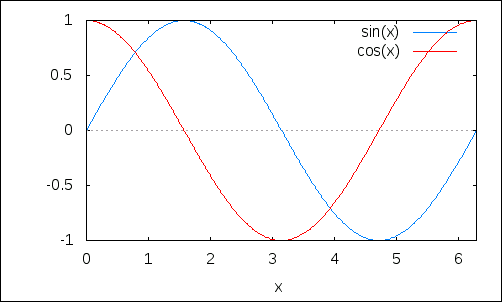
\includegraphics[width=9cm]{10minute_img/10minute_1.png}
\end{center}
\begin{center}
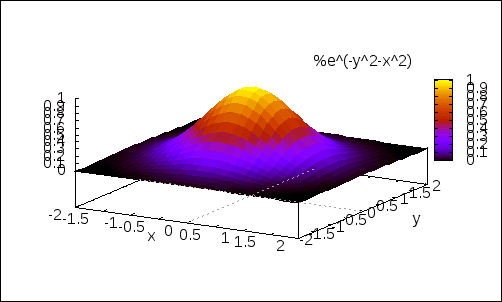
\includegraphics[width=9cm]{10minute_img/10minute_2.png}
\end{center}
``diff"함수를 써서 미분을 해보겠습니다. 


\begin{verbatim}
(%i147) f(x) := x^2 $
diff(f(x), x);
g(y) := sin(y)$
g(f(x));
diff( g(f(x)) , x);
\end{verbatim}
$$
2\,x\leqno{\tt (\%o148)  }
$$
$$
sin\left( {x}^{2}\right) \leqno{\tt (\%o150)  }
$$
$$
2\,x\,cos\left( {x}^{2}\right) \leqno{\tt (\%o151)  }
$$


헤헤, 예 맥시마는 체인룰\footnote{우리말로 뭐지요? 까먹었어요. ㅠ.ㅠ}
을 알고 있습니다.

마지막으로 2차 미분 방정식을 풀어보겠습니다.

$$y''(t) + omega^2 * y(t) = 0$$


\begin{verbatim}
(%i152) assume(omega > 0);
ode2( 'diff(y, t, 2) + omega^2 * y = 0, y, t );

ic2(%, t = 0, y = amp, 'diff(y,t) = 0 );
\end{verbatim}
$$
[redundant]\leqno{\tt (\%o152)  }
$$
$$
y=\%k1\,sin\left( \omega\,t\right) +\%k2\,cos\left( \omega\,t\right) \leqno{\tt (\%o153)  }
$$
$$
y=amp\,cos\left( \omega\,t\right) \leqno{\tt (\%o154)  }
$$


이제 아쉬운 작별입니다. 이제부터는 스스로 알아서 하시고요. 모르는 게 나오면
F1키 누르는 것 잊지마시고요. 

맥시마랑 wxMaxima랑 많이 사랑해주셔요.

\end{document}
